% latex $fileNameWithoutExt; dvisvgm $fileNameWithoutExt --bbox=papersize --font-form=ttf --precision=3 --optimize=collapse-groups,group-attributes,simplify-text,simplify-transform
\documentclass[tikz, border=8mm]{standalone}
\usetikzlibrary{matrix}
\usetikzlibrary{positioning}
\begin{document}
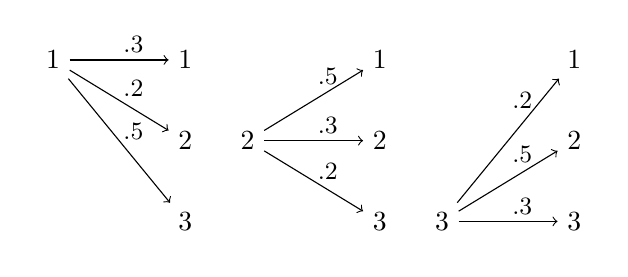
\begin{tikzpicture}
  \begin{scope}
    \matrix (m) [matrix of nodes, column sep=36px, row sep=16px]
    {
      1 & 1 \\
        & 2 \\
        & 3 \\
    };
    \path[->, font=\small]
    (m-1-1) edge node [above right=-1px and -2px] {.3} (m-1-2)
    (m-1-1) edge node [above right=-2px and -2px] {.2} (m-2-2)
    (m-1-1) edge node [above right=-3px and -2px] {.5} (m-3-2);
  \end{scope}
  \begin{scope}[xshift=70px]
    \matrix (m) [matrix of nodes, column sep=36px, row sep=16px]
    {
        & 1 \\
      2 & 2 \\
        & 3 \\
    };
    \path[->, font=\small]
    (m-2-1) edge node [above right= 2px and -2px] {.5} (m-1-2)
    (m-2-1) edge node [above right=-1px and -2px] {.3} (m-2-2)
    (m-2-1) edge node [above right=-3px and -2px] {.2} (m-3-2);
  \end{scope}
  \begin{scope}[xshift=140px]
    \matrix (m) [matrix of nodes, column sep=36px, row sep=16px]
    {
        & 1 \\
        & 2 \\
      3 & 3 \\
    };
    \path[->, font=\small]
    (m-3-1) edge node [above right= 8px and -2px] {.2} (m-1-2)
    (m-3-1) edge node [above right= 3px and -2px] {.5} (m-2-2)
    (m-3-1) edge node [above right=-1px and -2px] {.3} (m-3-2);
  \end{scope}
\end{tikzpicture}
\end{document}
